% Install the VS Code extension to view the PDF rendering in a tab
\documentclass{report}
\usepackage{fullpage}
\usepackage[T1]{fontenc}
\usepackage[mathletters]{ucs}
\usepackage[utf8x]{inputenc}
\setlength{\parskip}{.8em} 
\usepackage{graphicx}
\usepackage{listings}
\usepackage{color}

\definecolor{dkgreen}{rgb}{0,0.6,0}
\definecolor{gray}{rgb}{0.5,0.5,0.5}
\definecolor{mauve}{rgb}{0.58,0,0.82}
\graphicspath{ {./scatters/} }

\lstset{frame=tb,
	language=Java,
	aboveskip=3mm,
	belowskip=3mm,
	showstringspaces=false,
	columns=flexible,
	basicstyle={\small\ttfamily},
	numbers=none,
	numberstyle=\tiny\color{gray},
	keywordstyle=\color{blue},
	commentstyle=\color{dkgreen},
	stringstyle=\color{mauve},
	breaklines=true,
	breakatwhitespace=true,
	tabsize=3
}


\begin{document}
	\begin{flushleft}
		\huge CS 415 Project 1
		
		\normalsize Keegan Donley, Jeff Hultman

		\section{Task 1}

		\paragraph{Average-case efficiency of Euclid's algorithm and consecutive integer checking algorithm}
		To test the average-case efficiency of these algorithms, we generate 100 values of n from 1 to 70, then count the number of
		operations needed to calulate the average GCD for n using Euclid's algorithm and consecutive integer checking.

		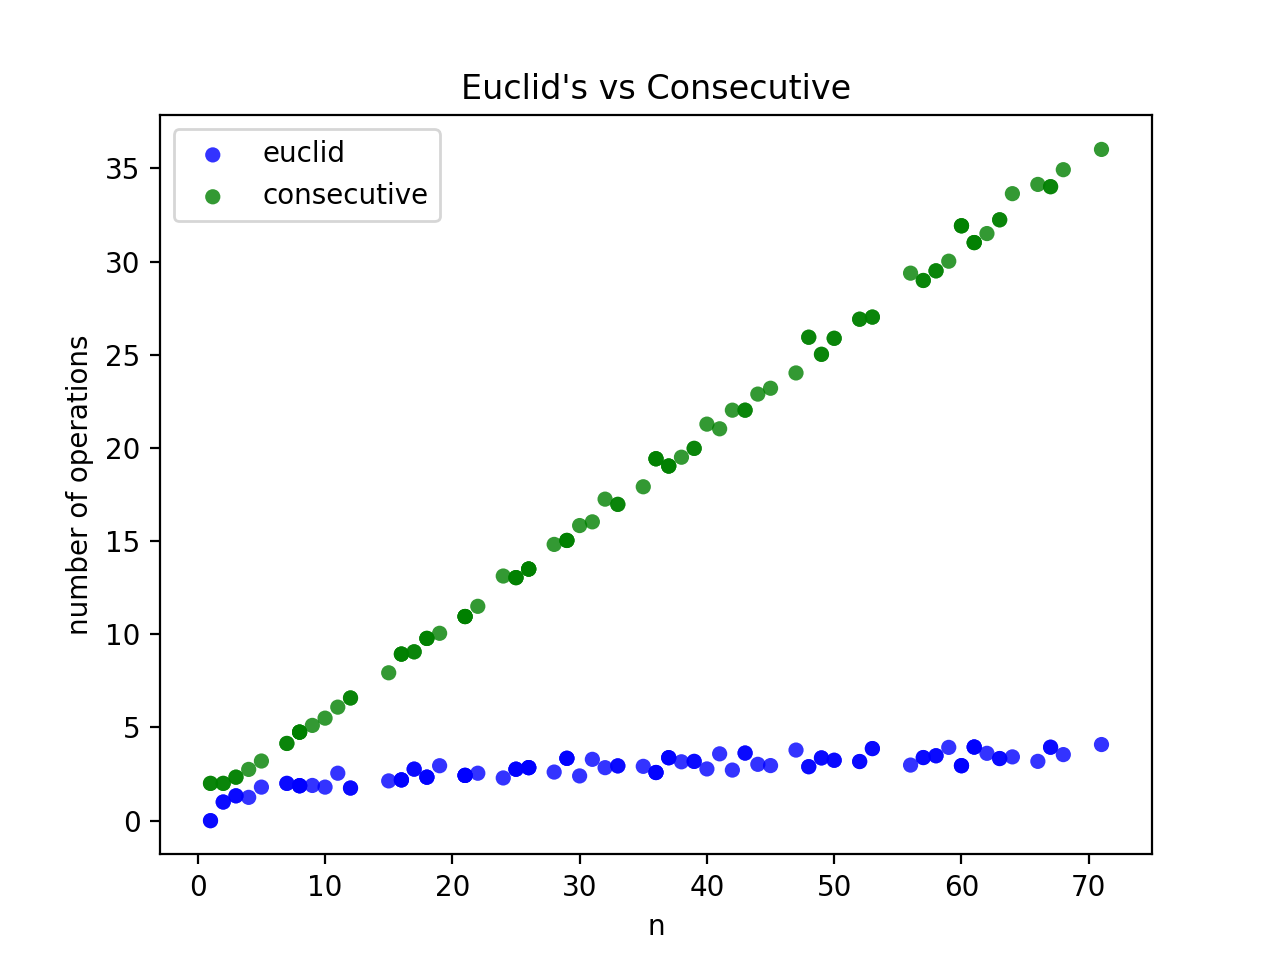
\includegraphics{task1}

		\textbf{Euclid} $\theta$(logn)
		
		\textbf{Consecutive Integer} $\theta$(n)

		\section{Task 2}

		\paragraph{Worst-case efficiency of Euclid's algorithm}
		The worst case for Euclid's algorithm occurs when two consecutive integers from the Fibonacci sequence are used as m and n.  

		\section{Task 3}

		\paragraph{The "middle-school procedure"}
		Information

	\end{flushleft}
\end{document}